\section{Auswertung}
\label{sec:auswertung}

\subsection{Fourier-Amplituden von drei verschiedenen Schwingungsformen} % (fold)
\label{sub:fourier_amplituden_von_drei_verschiedenen_}

\begin{figure}[!h]
	\centering
	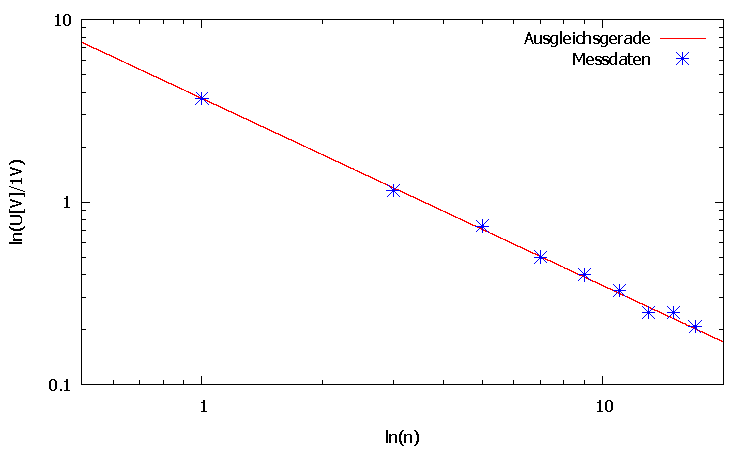
\includegraphics[width = 8cm]{img/rechteck.pdf}
	\caption{Graphische Darstellung der Fourier-Amplituden einer Rechteckspannung und einem 1/x fit.}
	\label{gra:recht}

	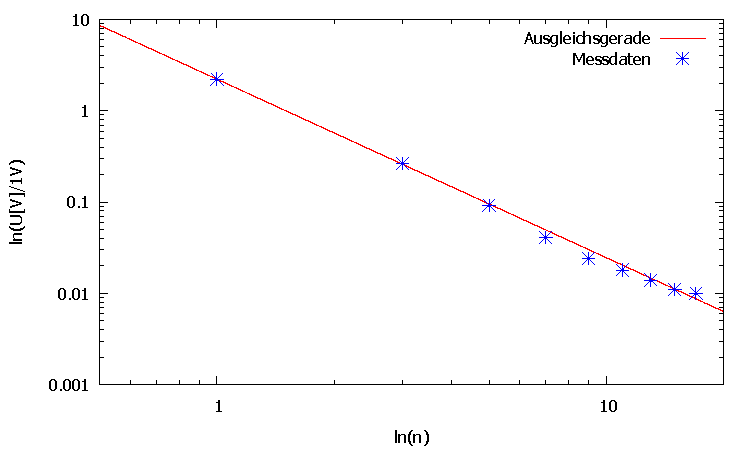
\includegraphics[width = 8cm]{img/dreieck.pdf}
	\caption{Graphische Darstellung der Fourier-Amplituden einer Dreiecksspannung und einem 1/$x^2$ fit.}
	\label{gra:dreieck}

	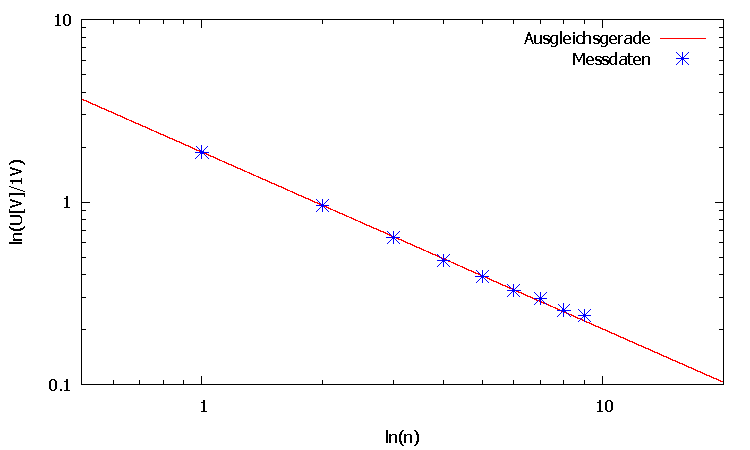
\includegraphics[width = 8cm]{img/saegezahn.pdf}
	\caption{Graphische Darstellung der Fourier-Amplituden einer S"agezahnspannung und einem 1/x fit.}
	\label{gra:saege}
\end{figure}

\clearpage


\begin{table}[!h]
\begin{center}
\begin{tabular}{|r|r|r|r|r|r|}
\hline
 Rechteck & & Saegezahn & & Dreieck & \\
 n-te Oberwelle & U[V] & n-te Oberwelle & U[V] & n-te Oberwelle & U[V] \\
\hline
\hline
1	& 3.700 & 1	& 1.880 & 1	& 2.220 \\
3	& 1.160 & 2	& 0.960 & 3	& 0.266 \\
5	& 0.740 & 3	& 0.640 & 5	& 0.092 \\
7	& 0.500 & 4	& 0.480 & 7	& 0.041 \\
9	& 0.400 & 5	& 0.392 & 9	& 0.024 \\
11	& 0.328 & 6	& 0.328 & 11& 0.018 \\
13	& 0.248 & 7	& 0.296 & 13& 0.014 \\
15	& 0.249 & 8	& 0.256 & 15& 0.011 \\
17	& 0.208 & 9	& 0.240 & 17& 0.010 \\
\hline
\end{tabular}
\caption[]{Messwerte der Spannung $U$ bei der n-ten Oberschwingung}
\label{tab:messwerte}
\end{center}
\end{table}


Bei der Messung der ersten 9 von null verschiedenen Fourieramplituden einer Rechtecks-, einer Dreiecks- und einer Saegezahnschwingung ergaben sich die in Tabelle \ref{tab:messwerte} gemessen Werte. Die Daten sind in den Graphiken \ref{gra:recht}, \ref{gra:dreieck} und \ref{gra:saege} dargestellt.

Die Fourierkoeffizienten der Funktionen wurden nach den Gleichungen \eqref{eqn:a_n} und \eqref{eqn:b_n} errechnet und lauten:

\begin{eqnarray*}
\text{Rechteck}: b_\mathrm{n} &=& \frac{4}{n \pi}, n \, \text{ungerade} \qquad ,\\
\text{S"agezahn}: b_\mathrm{n} &=& \frac{\pi^2}{n}  \qquad ,\\
\text{Dreieck}: a_\mathrm{n} &=& \frac{4}{n^2 \pi^2}, n \,\text{ungerade} \qquad .\\
\end{eqnarray*}

Bei der Rechtecks- und S"agezahnspannung ist eine erwartete Abnahme der Amplitude mit 1/x erkennbar.
Die Dreiecksspannung hingegen l"asst eine erwartete 1/$x^2$ Abh"angigkeit erkennen.

Eine Ausgleichsrechnung mithilfe der Funktion $a/(x+b)$ bzw. $a/(x+b)^2$ ergab folgende Werte:

\begin{table}[!h]
\begin{center}
\begin{tabular}{|r|r|r|r|r|r|}
\hline
Dreieck & & Rechteck & & S"agezahn &\\
a & b & a & b & a & b\\
\hline
\hline
2.43 & 0.05 & 3.49 & -0.06 & 1.98 & 0.06\\
\hline
\end{tabular}
\label{}
\end{center}
\end{table}

Da die Punkte alle auf dem Fit liegen, jedoch $b \neq 0$ ist, scheinen systematische Fehler vorzuliegen. Dies k"onnte an den Analyse Bauteilen des Oszilloskops liegen, sodass eine minimale Verschiebung entsteht.

\subsection{Sukzessive Zusammensetzung verschiedener Schwingungsformen aus deren Komponenten} % (fold)
\label{sub:sukzessive_zusammensetzung_verschiedener_schwingungsformen_aus_deren_komponenten}

\begin{figure}[!h]
	\centering
	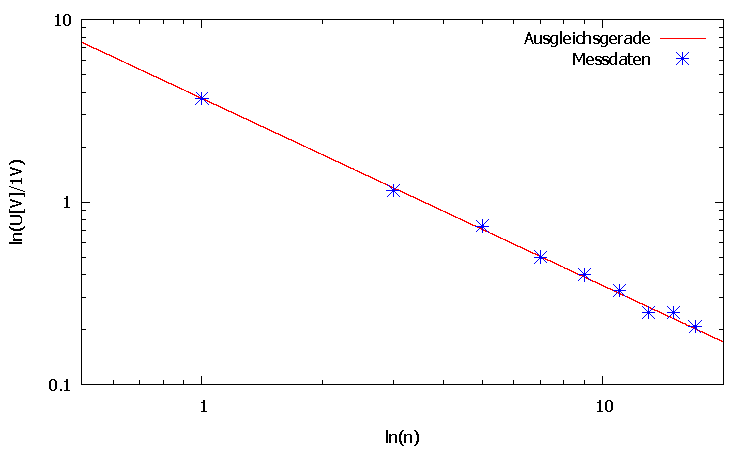
\includegraphics[width = 8cm]{img/rechteck.pdf}
	\caption{Fouriersynthese einer Rechteckspannung aus den ersten 9 Oberschwingungen.}
	\label{fg:recht}

	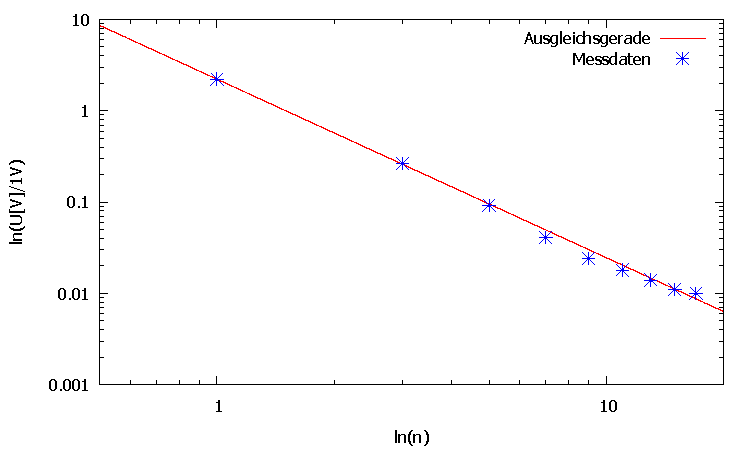
\includegraphics[width = 8cm]{img/dreieck.pdf}
	\caption{Fouriersynthese einer Dreiecksspannung aus den ersten 9 Oberschwingungen.}
	\label{fg:dreieck}

	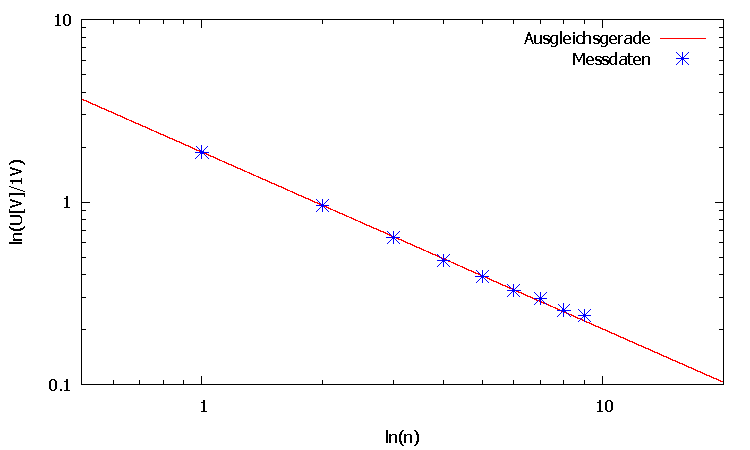
\includegraphics[width = 8cm]{img/saegezahn.pdf}
	\caption{Fouriersynthese einer S"agezahnspannung aus den ersten 9 Oberschwingungen.}
	\label{fg:recht}
\end{figure}